\documentclass{report}
\usepackage{hyperref}
\usepackage{fontspec}
\usepackage{amsmath} 
\usepackage{graphicx}
\usepackage{nopageno}
\usepackage{courier}
\usepackage{listings}
\usepackage{parskip}
\usepackage{framed}
\usepackage{tikz}
\usetikzlibrary{arrows,positioning}
%\usepackage{ulem}
\setmonofont{Noto Mono}
%\newfontfamily{\Courier}{Nimbus Mono PS}
%\setmainfont{AR PL UKai TW}
\setmainfont{Times New Roman}
\renewcommand{\ttdefault}{pcr}
\XeTeXlinebreaklocale "zh"
\usepackage[a4paper, total={6in, 8in}]{geometry}
\pagestyle{plain}
\newcommand{\bs}{\textbackslash}

\usepackage{xcolor}
\usepackage{listings}
\definecolor{mGreen}{rgb}{0.2,0.8,0.2}
\definecolor{mGray}{rgb}{0.5,0.5,0.5}
\definecolor{mRed}{rgb}{0.58,0,0.82}
\definecolor{backgroundColour}{rgb}{0,0,0}
\definecolor{mWhite}{rgb}{0.9,0.9,0.9}
\lstset{basicstyle=\ttfamily}
\lstdefinestyle{CStyle}{
    backgroundcolor=\color{backgroundColour},   
    commentstyle=\color{mGray},
    keywordstyle=\color{mGreen},
    numberstyle=\color{mGray},
    stringstyle=\color{mRed},
    basicstyle=\color{mWhite},
    breakatwhitespace=false,         
    breaklines=true,                 
    captionpos=b,                    
    keepspaces=true,                 
    numbers=left,                    
    numbersep=5pt,                  
    showspaces=false,                
    showstringspaces=false,
    showtabs=false,                  
    tabsize=2,
    language=C
}

\title{A Handout For Students in Kan Chiao}
\author{Handsome Liu}

\begin{document}
\fontsize{12pt}{16pt}\selectfont
\maketitle
\tableofcontents
\part{Introduction}
\chapter{C/C++ Programming Language}
\section{Programming Language}
\subsection{Programming Language and Natural Language}

    Different from \textbf{natural language}, the language that we using to communicate with other \textit{human beings}, \textbf{programming language} is a kind of language that we using to communicate with \textit{machines}.

    As you may expect, computers are not smart enough to comprehend C/C++ programming language directly. The language used by CPUs is called \textit{machine code}. As a result, we need a \textbf{compiler} to achieve such translation. The concept of \textbf{compile} and \textbf{interpret} will be introduced in later section.\\

    \begin{framed}
    \begin{center}
    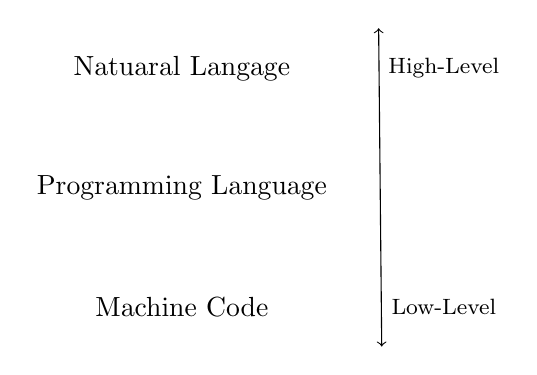
\begin{tikzpicture}[node/.style={rectangle,minimum height=10mm},node distance=5mm]
    \node(nl)[node]   {Natuaral Langage};
    \node(pl)[node,below= of nl]   {Programming Language};
    \node(mc)[node,below= of pl]   {Machine Code};
    \node(hl)[node,right=1cm of nl]   {\footnotesize High-Level};
    \node(ml)[node,below= of hl]   {};
    \node(ll)[node,below= of ml]   {\footnotesize Low-Level};
    \draw [<->] (hl.north west)--(ll.south west);
    \end{tikzpicture}
    \end{center}
    \end{framed}
    
\subsection{Source File}
    The code you wrote is called the \textbf{source code}, and the file containing your source code is called the \textbf{source file}.

\subsection{Compile and Interpret}

    To \textbf{compile} means to translate \textit{the whole source file} into another language, say, machine code.

    To \textbf{interpret} means to translate the source code \textit{line by line} and execute it immediately.

    Programming languages that needs to be compiled are called \textbf{compiled language}, while those that needs to be interpreted are called \textbf{interpreted language}.

\section{C/C++ Language}
    
    C programming language is a programming language developed by \textit{Dennis Ritchie} in 1969 ~ 1973. It is general-purpose, efficient and easy-to-read, which makes it the first choice for informatics competition.

    Based on the syntax of C, \textit{Bjarne Stroustrup} create C++ programming language to achieve \textit{OOP (object-oriented programming)}. 
    
    \subsection{Source File and Header File}

    Sometimes, it's kind of stupid to define all things in a single file. In C/C++, you can define things in some other files. The file that contains the \texttt{main()} function is called \textbf{source file}, and the files you used to define things in them are called \textbf{header files}. In this book, we will not learn how to write your own header files, but we will learn how to use others' header files.

    \subsection{Compiler for C/C++}

    C and C++ are both \textbf{compiled languages}, which means we need a compiler to compile your source code in order to execute it. The most-used one in Windows system is called \texttt{mingw}, while the most-used one in Linux system is called \texttt{gcc}.

\section{IDE (Intergrated Development Environment)}

    IDE is a kind of application that provides facilities to programmers for coding. An IDE usually consists of:
    \begin{itemize}
    \item a code editor (with syntax highlighter)
    \item automatically building tools (call the compiler to compile your source code, and execute it automatically)
    \item a debugger (tells you which line of your code disobeys the rule of syntax)
    \end{itemize}

    \subsection{Code::Blocks}

    \textit{Code::Blocks} is a free, open-source IDE that supports many programming languages. Actually, Code::Blocks itself is developed in C++.

\section{Run on Your PC}

    \subsection{IDE and Compiler Installation}
    
    Go to \url{http://www.codeblocks.org/downloads/26}.

    If you are using Windows, please choose \textit{codeblocks-xx.xxmingw-setup.exe}.

    If you are using Linux, please choose the one corresponding the operating system you use.
        
    If you are using Mac, you don't have any choice, just press the only link for Mac OS X.

    After downloading, follow the installation guide until the installation is complete.

    \subsection{Test}

    After finishing the installation, press \texttt{Ctrl+Shift+N} to open a new file. Paste the code below, and press the button with gear and green triangle to execute it.

\begin{lstlisting}[style=CStyle]
#include<stdio.h>
int main(){
    printf("Handsome Liu is so handsome!\n");
}
\end{lstlisting}

    If you've done all the steps above correctly, you should see a windows with text \texttt{ Handsome Liu is so handsome! } on it. However, if there is not, please check all the steps again.

\part{Getting Started}
\chapter{Basic Concepts}
    In this chapter, we will introduce some basic concepts you need to know.
    \section{}
\end{document} 
